\chapter{Significance of \jwone and \jwtwo for GK stars}\label{chap:3}
% TEXT ==========================================

We identify by eye from the median color plots (e.g., Figures \ref{fig:median_stick_bar_jw1} and \ref{fig:median_stick_bar_jw1}) for all WISE/2MASS colors that \jwone and \jwtwo present a significant separation in color between dwarfs and (sub-)giants for all G and early K spectral types. This trend in \jwone and \jwtwo with luminosity class for G and early K dwarfs may extend to later spectral types (M stars), but the limited number of M dwarfs in the Michigan Spectral Atlases precludes a robust determination.

The separation is approximately one robust standard deviation of the colors for a given spectral type and luminosity class. For example, the color distribution of G5V stars is $J-W2=0.405\pm0.078$, for G5III stars is $J-W2=0.573\pm0.055$, a difference of $0.168\pm0.095$ of more than one standard deviation. While there is significant overlap in the colors of stars of different luminosity classes, this still permits a probabilistic assignment of luminosity class which we explore further in Chapter \ref{chap:4}.

The robust standard deviation of the colors of a given spectral type and luminosity class in the spectral type range of interest (G0-K5) is consistent with typical WISE and 2MASS magnitude measurement uncertainties ($\sim$0.05--0.15 mag). Thus, this implies the overlap in the dwarf-giant color distributions may be due to measurement uncertainties rather than a physical origin.  More precise color measurements may increase the statistical significance of this separation between dwarfs and (sub-)giants in color. How to utilize color separation, also seen in the color probability functions created in Chapter \ref{subsec:tdist_stats}, is discussed and visualized in specific detail in Chapter \ref{sec:color_prob_func}. 

In the next sections, we turn to highlighting sample applications of utilizing this primary result for use in distinguishing dwarfs from giants.

\section{Possible origins of dwarf-giant color separation}

We have considered two possibilities for this observable difference in the infrared colors of dwarf stars compared to giant stars. We have considered that the source of the color difference is due to (1) observational bias from reddening due to galactic extinction, or is (2) astrophysical in origin, which would help underline the intrinsic physical difference of dwarfs from giant stars. We stipulate that while there is a possibility both (1) and (2) could be contributing to the color difference we do see among different luminosity classes, it is more likely that (2) is the more dominant effect, which has interesting astrophysical implications in characterizing dwarfs from giants stars. 

We infer that (2) is more likely than (1) because we have examined the medians magnitudes of colors, for which we had greatest separation (\jwone and \jwtwo), across the galactic latitude coordinate $b$. We consider $b$ since it can assess whether galactic extinction may have contributed more reddened colors that could have explained this color separation (Figure \ref{fig:color-vs-b}). We estimate that any reddening effect due to extinction should be strongest at the sky area that covers the galactic plane where gas clouds are concentrated, at approximately $|b|<15$. Median color does not typically spike in the galactic plane for both \jwone and \jwtwo while in the same luminosity group (Figure \ref{fig:color-vs-b}), which suggests that the color separation between dwarfs and giants is not due to extinction, but from astrophysical cause, such as gravity-sensitive lines in J-band.

% FIGURES ==========================================

\begin{figure}
    \centering
    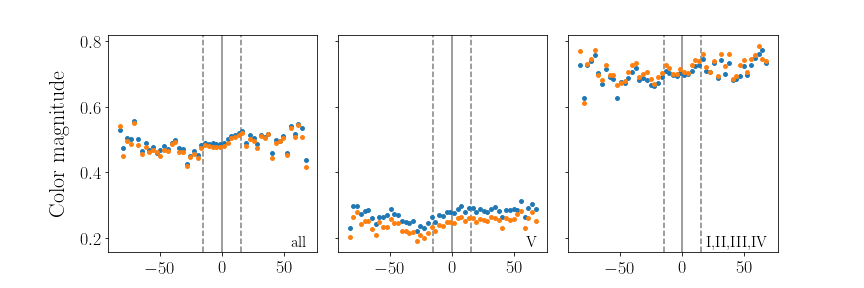
\includegraphics[width=1.0\textwidth,clip=true]{Figures/populations/plot-b-vs-color.png}
    \caption{This figure displays the median values of color magnitude \jwone and \jwtwo across galactic latitude for different luminosity classes. Colors magnitude and luminosity class information originate from a cross-matched table of WISE/2MASS with the Michigan Spectral Atlas, and no extinction correction has been applied. There is no considerable reddening of color for latitudes that contain the galactic plane ($|b|<15$), which suggests the color separation is not extinction dependent.}
    \label{fig:color-vs-b}
\end{figure}